%
% phianalysis.tex -- Average
%
% (c) 2019 Prof Dr Andreas Müller, Hochschule Rapperswil
%

\begin{frame}[fragile]
\frametitle{Averaging}

\begin{center}
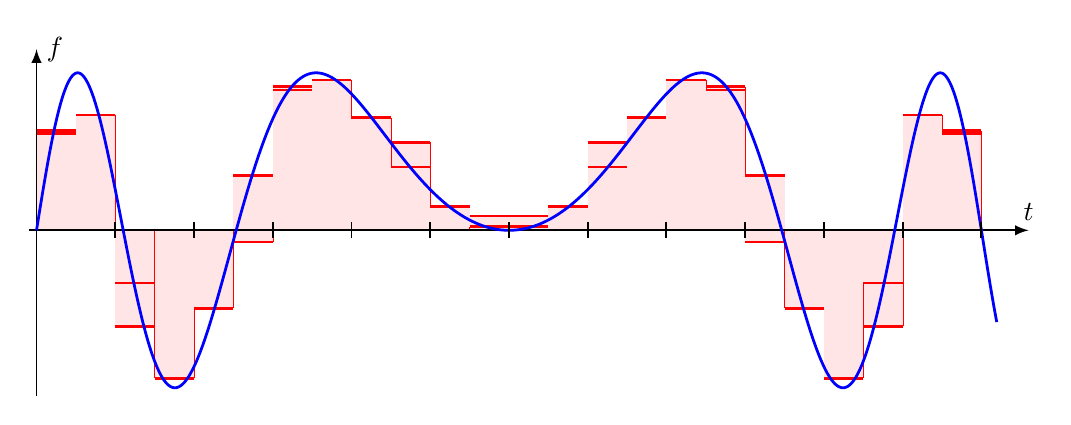
\begin{tikzpicture}[>=latex]

	\def\punkt#1#2#3{
		2*sin(15*(#1*#3+(1-#3)*#2)*(12-(#1*#3+(1-#3)*#2)))
	}

	\def\stufe#1#2{
		\pgfmathparse{
			0.090909*(\punkt{#1}{#2}{1}+\punkt{#1}{#2}{0.1}+\punkt{#1}{#2}{0.2}+\punkt{#1}{#2}{0.3}+\punkt{#1}{#2}{0.4}+\punkt{#1}{#2}{0.5}+\punkt{#1}{#2}{0.6}+\punkt{#1}{#2}{0.7}+\punkt{#1}{#2}{0.8}+\punkt{#1}{#2}{0.9}+\punkt{#1}{#2}{0})
		}
		\xdef\y{\pgfmathresult}
		\draw[color=red,line width=0.1pt] (#1,0)--(#1,\y);
		\draw[color=red,line width=0.1pt] (#2,0)--(#2,\y);
		\fill[color=red!10] (#1,0)--(#2,0)--(#2,\y)--(#1,\y)--cycle;
		\draw[color=red,line width=1pt] (#1,\y)--(#2,\y);
	}

	\begin{scope}
		\clip (-0.1,-2.1) rectangle (12.3,2.1);
		\foreach \x in {1,...,12}{
			\pgfmathparse{\x-1}
			\xdef\xlinks{\pgfmathresult}
			\pgfmathparse{\x}
			\xdef\xrechts{\pgfmathresult}
			\only<\x>{ \stufe{\xlinks}{\xrechts} }
		}
		\foreach \x in {13,...,36}{
			\pgfmathparse{(\x-13)*0.5}
			\xdef\xlinks{\pgfmathresult}
			\pgfmathparse{(\x-12)*0.5}
			\xdef\xrechts{\pgfmathresult}
			\only<\x>{ \stufe{\xlinks}{\xrechts} }
		}
	\end{scope}

	\draw[->,line width=0.7pt] (-0.1,0)--(12.6,0)
		coordinate[label={$t$}];
	\draw[->,line width=0.7pt] (0,-2.1)--(0,2.3)
		coordinate[label={right:$f$}];

	\draw[color=blue,line width=1pt] plot[domain=0:12.2,samples=1000]
		({\x},{2*sin(15*\x*(12-\x))});

	\foreach \x in {1,...,12}{
		\draw[line width=0.7pt] ({\x},-0.1)--({\x},0.1);
	}

\end{tikzpicture}
\end{center}

\begin{align*}
f(t) &\simeq
\only<1-12>{
	\uncover<1->{  a_{0,0}  T_0\phi(t) +\mathstrut}
	\uncover<2->{  a_{0,1}  T_1\phi(t) +\mathstrut}
	\uncover<3->{  a_{0,2}  T_2\phi(t) +\mathstrut}
	\uncover<4->{  a_{0,3}  T_3\phi(t) +\mathstrut}
	\uncover<5->{  a_{0,4}  T_4\phi(t) +\dots}
}
\only<13-36>{
	\uncover<13->{ a_{1,0} D_{\frac12}T_0\phi(t)+\mathstrut }
	\uncover<14->{ a_{1,1} D_{\frac12}T_1\phi(t)+\mathstrut }
	\uncover<15->{ a_{1,2} D_{\frac12}T_2\phi(t)+\mathstrut }
	\uncover<16->{ a_{1,3} D_{\frac12}T_3\phi(t)+\dots }
}
\\
&
\only<1-12>{=
	\uncover<6->{
		\sum_{k\in\mathbb Z} a_{0,k} T_k\varphi(t)
	}
}
\only<13-36>{=
	\uncover<17->{
		\sum_{k\in\mathbb Z} a_{1,k} D_{\frac12}T_k\varphi(t)
	}
}
\end{align*}

\end{frame}





